\section[Diffeomorphismen, implizite Funktionen, Rang]{Diffeomorphismen, Umkehrsatz, Satz über implizite Funktionen und Abbildungen von konstantem Rang}
\Einleitung{Letztes Mal hatten wir uns insbesondere Funktionen $F:\mathbb{R}^n\supseteq U\to\mathbb{R}$ angeschaut und viele der Eigenschaften wiederentdeckt, die wir schon von $f:\mathbb{R}\to\mathbb{R}$ kannten (Extrema, Mittelwertsatz, Taylorentwicklung, Verkettung).\\
Für eindimensionale Funktionen haben wir deren Umkehrabbildungen $f^{-1}$ und Kriterien, wann diese überhaupt existieren, kennengelernt.\\
Wie sehen diese aber für Abbildungen $\Fvec:U\to V$ zwischen offenen Teilmengen $U,V$ des $\mathbb{R}^n$ aus?\\
Welche Eigenschaften bringen sie mit sich, was muss man beachten?\\
Zudem kommt ein wichtiger, auf den ersten Blick aber komplexer Satz auf euch zu: Der Satz über implizite Funktionen.\\
Abschließend schauen wir noch, wie wir Funktionen mithilfe des Differentials anhand des Ranges charakterisieren können. Das ist vor allem im Hinblick auf Untermannigfaltigkeiten wichtig.}

\subsection{Diffeomorphismen: Umkehren in höheren Dimensionen}
\begin{Def}{Diffeomorphismus}
Eine Abbildung zwischen \underline{offenen Teilmengen} $U$ und $V$ des $\mathbb{R}^n$ nennen wir \red{Diffeomorphismus}, wenn $\Fvec:U\to V$ \underline{bijektiv} und \underline{stetig differenzierbar} ist mit einer ebenso \underline{stetig differenzierbaren} Umkehrabbildung.
\end{Def}
\begin{Beispiel}
{Bekannter Diffeomorphismus}
Die Abbildung $f:\mathbb{R}\to\mathbb{R}_+\setminus\MengeDirekt{0},\,f(x)=e^x$ ist mit $f^{-1}:\mathbb{R}_+\setminus\MengeDirekt{0}\to\mathbb{R},\,f^{-1}(x)=\ln(x)$ ein Diffeomorphismus, denn beide sind stetig differenzierbar, bijektiv und\\
$(f\circ f^{-1}=\Id_{\mathbb{R}_+\setminus\MengeDirekt{0}})\land (f^{-1}\circ f=\Id_\mathbb{R}).\,\checkmark$
\end{Beispiel}

Für die folgenden Betrachtungen wird es nützlich sein, die folgenden elementaren Begriffe griffbereit zu haben:
\begin{Wiederholung}
{Injektivität{,} Surjektivität}\label{wdh:09InjekSurjek}
Für Abbildungen $f:A\to B$ hatten wir definiert:
\begin{align*}
        f\tx{ ist \red{surjektiv}.}&\iff \tx{Die gesamte Bildmenge wird getroffen.}\\
        &\iff f(A)=B\\
        &\iff \forall b\in B\exists a\in A: f(a)=b\\
        f\tx{ ist \red{injektiv}.}&\iff\tx{Jedes Bild hat genau ein Urbild.}\\
        &\iff\forall b\in f(A)\exists!a\in A: f(a)=b\\
        &\iff \forall x,y\in A: f(x)=f(y)\implies x=y\\
        \tx{ ist \red{bijektiv}.}&\iff f\tx{ ist injektiv und surjektiv.}
\end{align*}
\end{Wiederholung}
\begin{Wiederholung}
{Lemma zur Bijektivität und Umkehrabbildung}\label{wdh:09BijektivitatUmkehrabbildung}
Eine Abbildung $f:A\rightarrow B$ ist \underline{genau dann bijektiv}, falls es eine Abbildung $g:B\to A$ gibt (diese nennen wir dann \red{Umkehrabbildung}), die die folgenden Relationen erfüllt:
\begin{equation}
    g\circ f=\text{Id}_A\,\wedge\, f\circ g=\text{Id}_B.\label{eq:Umkehrabbildung}
\end{equation}
\end{Wiederholung}
\begin{Satz}{Satz}
{Zum Differential der Umkehrabbildung}
Ist $\fvec:U\to V$ ein Diffeomorphismus, so folgt:\\
Das Differential $d\fvec_\xvec$ ist für alle $\xvec\in U$ differenzierbar und es gilt
\begin{equation}
    (d\fvec^{-1})_{\fvec(\xvec)}=(d\fvec_\xvec)^{-1}.
\end{equation}
Den analogen Satz (Ableitung der Umkehrfunktion) hatten wir auch schon in MfP1 für 1D-Funktionen.
\end{Satz}
Diese Aussage ist auf den ersten Blick vielleicht nicht ganz klar, daher ein Beispiel:
\begin{Beispiel}
{Ausführliches Beispiel zu umkehrbaren Abbildungen}
Wir definieren $U:=\mathbb{R}\times\BracedIn{-\frac{\pi}{2},\frac{\pi}{2}}$ und $V:=(0,\infty)\times \mathbb{R}$.\\
Sei nun $\hvec:U\to V,\,\boxed{\hvec(u,v)=\MatrixInline{e^u\cos(v)\\e^u\sin(v)}}$.\\
Warum ist dies ein Diffeomorphismus?
\begin{itemize}
    \item \textbf{Stetige Differenzierbarkeit}:\\
    Wir stellen fest, dass $\hvec$ stetig differenzierbar ist, da \underline{alle} partiellen Ableitungen stetig sind.
    \item \textbf{Bijektivität}:
    \begin{itemize}
        \item Für die Injektivität nutzen wir die dritte Äquivalenz (siehe \hyperref[wdh:09InjekSurjek]{Wdh. 9.1}) und zeigen, dass die Gleichheit des Bildes die Gleichheit des Urbildes impliziert:\\
        Seien $(u,v)$ und $(u',v')\in U$ mit $\hvec(u,v)=\hvec(u',v')$.\\
        Ist $\hvec$ injektiv, muss jetzt also folgen, dass $(u,v)=(u',v')$.\\
        Aus den Komponenten von $\hvec$ ergeben sich die beiden Gleichungen
        \begin{align*}
            e^u\cos(v)&=e^{u'}\cos(v'),\quad e^u\sin(v)=e^{u'}\sin(v').
        \end{align*}
        Weil $\cos(v)\neq0\forall v\in\BracedIn{-\frac{\pi}{2},\frac{\pi}{2}}$ ist, können wir die erste Gleichung durch $\cos(v)$ teilen und dann $e^u$ in die zweite Einsetzen, sodass wir
        \begin{equation*}
            e^{u'}\frac{\sin(v)}{\cos(v)}\cos(v')=e^{u'}\sin(v')\overset{e^{u'}\neq0}{\iff}\tan(v)=\tan(v').
        \end{equation*}
        Da $\tan(v)$ auf dem Intervall für $v$ bzw $v'$ injektiv ist, folgt $v=v'$. Aus der ersten Gleichung folgt dann aber auch, dass $e^{u}=e^{u'}$ und aus der Injektivität der $e$-Funktion $u=u'$.\\
        Es gilt also $\hvec(u,v)=\hvec(u',v')\implies(u,v)=(u',v')\iff\hvec$ ist injektiv.
        \item Für die Surjektivität müssen wir zeigen, dass $(0,\infty)\times\mathbb{R}$ tatsächlich das Bild von $\hvec$ ist.\\
        Dies wird bei Betrachtung der Komponenten deutlich, denn es sind
        \begin{align*}
            \inf(e^u\cos(v))&=0,\quad\sup (e^u\cos(v))=\infty,\\
            \inf(e^u\sin(v))&=-\infty,\quad\sup (e^u\sin(v))=\infty.
        \end{align*}
    \end{itemize}
    Alternativ eignet sich sonst auch das \hyperref[wdh:09BijektivitatUmkehrabbildung]{Lemma zur Bijektivität und Umkehrabbildung}, welches gerade im Kontext von Diffeomorphismen nützlich ist, da wir diese Relationen sowieso zeigen müssen.
    \item \textbf{Umkehrabbildung finden}:\\
    Um die Umkehrabbildung zu finden, eignen sich zwei Strategien:
    \begin{itemize}
        \item Raten und Ausprobieren (gerade bei einfacheren Abbildungen).
        \item Ein Gleichungssystem aufstellen und Invertieren.\footnote{Wie wir es aus 1D kennen, z. B. $y=2e^{-\frac{x}{4}}\iff x=-4\BracedIn{\ln(y)-\ln(2)}.$}
    \end{itemize}
    Wir wenden die zweite Methode an und haben somit das Gleichungssystem
    \begin{align*}
        x&=e^u\cos (v)\\
        y&=e^u\sin(v).
    \end{align*}
    Dieses wollen wir nun nach $u$ und $v$ auflösen. Indem wir die beiden Gleichungen durcheinander teilen, haben wir
    \begin{equation*}
        \iff\frac{y}{x}=\tan(v)\iff v=\arctan\BracedIn{\frac{y}{x}}\implies u=\ln\BracedIn{\frac{y}{\sin(\arctan(y/x))}}.
    \end{equation*}
    \blue{\textbf{Nebenrechnung}:\\
    Der Ausdruck für $u$ ist ziemlich sperrig - trigonometrische Überlegungen helfen bei der Vereinfachung:\\
    In einem rechtwinkligen Dreieck gilt $\alpha=\arcsin\BracedIn{\frac{b}{c}}$ (I) und $\alpha=\arctan\BracedIn{\frac{b}{a}}$ (II).\\
    Der Satz des Pythagoras besagt zudem, dass $c=\sqrt{a^2+b^2}$ (III).\\
    Setzen wir nun (I) $=$ (II), so erhalten wir
    \begin{equation}\label{eq:09HilfeTrigo}
        \arcsin\BracedIn{\frac{b}{c}}=\arctan\BracedIn{\frac{b}{a}}\iff\sin\BracedIn{\arctan\BracedIn{\frac{b}{a}}}=\frac{b}{c}\overset{(\III)}{=}\frac{b}{\sqrt{a^2+b^2}}.
    \end{equation}}
    Also ist (mit $a=x$ und $b=y$) der Ausdruck für $u$ schlicht
    \begin{equation*}
        u=\ln\BracedIn{\frac{y}{\sin(\arctan(y/x))}}\overset{\eqref{eq:09HilfeTrigo}}{=}\ln\BracedIn{\frac{y}{y/\sqrt{x^2+y^2}}}=\ln\BracedIn{\sqrt{x^2+y^2}}=\frac{1}{2}\ln(x^2+y^2).
    \end{equation*}
    Insgesamt lautet unsere Umkehrabbildung also
    \begin{equation*}
        \hvec^{-1}:(0,\infty)\times \mathbb{R}\to\mathbb{R}\times\BracedIn{-\frac{\pi}{2},\frac{\pi}{2}},\,\hvec^{-1}(x,y)=\MatrixInline{\frac{1}{2}\ln(x^2+y^2)\\\arctan\BracedIn{\frac{y}{x}}}.
    \end{equation*}
    \item \textbf{Umkehrabbildung bestätigen}:\\
    Ist dies nun wirklich die gewünschte Umkehrabbildung? Wir müssen die im Lemma gegebenen Relationen zeigen:
    \begin{eqnarray*}
        (\hvec\circ \hvec^{-1})(x,y)&\overset{\footnote{Einsetzen in $\hvec^{-1}$}}{}&\hvec\BracedIn{\frac{1}{2}\ln(x^2+y^2),\,\arctan\BracedIn{\frac{y}{x}}}\overset{\footnote{Einsetzen in $\hvec$}}{=}\MatrixInline{\exp\BracedIn{\frac{1}{2}\ln\BracedIn{x^2+y^2}}\cos\BracedIn{\arctan\BracedIn{\frac{y}{x}}}\\\exp\BracedIn{\frac{1}{2}\ln\BracedIn{x^2+y^2}}\sin\BracedIn{\arctan\BracedIn{\frac{y}{x}}}}\\
        &\overset{\footnote{Identitäten einsetzen (analog zur Nebenrechnung oben)}}{=}& \MatrixInline{\sqrt{x^2+y^2}\frac{x}{\sqrt{x^2+y^2}}\\\sqrt{x^2+y^2}\frac{y}{\sqrt{x^2+y^2}}}=\MatrixInline{x\\y}\,\checkmark\\
        (\hvec^{-1}\circ \hvec)(u,v)&=&\hvec^{-1}\BracedIn{e^u\cos(v),\,e^u\sin(v)}=\MatrixInline{\frac{1}{2}\ln\BracedIn{e^{2u}\cos^2(v)+e^{2u}\sin^2(v)}\\
        \arctan\BracedIn{\frac{e^u\sin(v)}{e^u\cos(v)}}}\\
        &\overset{\footnote{Nutze $\sin^2(v)+\cos^2(v)=1$}}{=}&\MatrixInline{\frac{1}{2}\ln\BracedIn{e^{2u}}\\\arctan(\tan(v))}=\MatrixInline{u\\v}.\,\checkmark
    \end{eqnarray*}
    Da $\hvec^{-1}$ \underline{stetig differenzierbar} und $\hvec$ nach dem obigen Lemma \underline{bijektiv} ist, ist $\hvec$ also ein Diffeomorphismus.
    \item \textbf{Anwendung des Satzes}:
    Laut dem Satz zum Differential der Umkehrabbildung gilt:
    \begin{equation*}
        (d\hvec^{-1})_{\hvec(u,v)}=\BracedIn{d\hvec}^{-1}_{(u,v)}.
    \end{equation*}
    Das wollen wir nun überprüfen:
    \begin{itemize}
        \item Linke Seite (zunächst für beliebige $(x,y)\in V$):
        \begin{eqnarray*}
            (d\hvec^{-1})_{(x,y)}&=&\MatrixInline{\grad(h_1^{-1})^T\\\grad(h_2^{-1})^T}=\MatrixInline{\partial_x\BracedIn{\frac{1}{2}\ln\BracedIn{x^2+y^2}}&\partial_y\BracedIn{\frac{1}{2}\ln\BracedIn{x^2+y^2}}\\\partial_x\BracedIn{\arctan\BracedIn{\frac{y}{x}}}&\partial_y\BracedIn{\arctan\BracedIn{\frac{y}{x}}}}\\
            &\overset{\footnote{Die Ableitung von $\arctan(x)$ können wir mit dem Satz über die Ableitung der Umkehrfunktion bestimmen:\\
            $y=\arctan(x)\iff \tan(y)=x\iff y'(x)(\tan^2(y)+1)=1\iff y'(x)=\frac{1}{x^2+1}$, wobei wir $(\tan'(y))=\tan^2(y)+1$ und die Kettenregel genutzt haben.}}{=}&\MatrixInline{\frac{x}{x^2+y^2}&\frac{y}{x^2+y^2}\\-\frac{y}{x^2}\frac{1}{1+y^2/x^2}&\frac{1}{x}\frac{1}{1+y^2/x^2}}=\frac{1}{x^2+y^2}\Matrix{x&y\\-y&x}.
        \end{eqnarray*}
        Auswerten bei $(x,y)=\hvec(u,v)=(e^u\cos(v),\, e^u\sin(v))$:\\
        Hier ist $\frac{1}{x^2+y^2}=\frac{1}{e^{2u}\BracedIn{\cos^2(v)+\sin^2(v)}}=e^{-2u}$:
        \begin{equation*}
            (d\hvec^{-1})_{\hvec(u,v)}=e^{-2u}e^u\MatrixInline{\cos(v)&\sin(v)\\-\sin(v)&\cos(v)}=e^{-u}\MatrixInline{\cos(v)&\sin(v)\\-\sin(v)&\cos(v)}.
        \end{equation*}
        \item Rechte Seite (zunächst die nicht Invertierte Matrix):
        \begin{equation*}
            d\hvec_{(u,v)}=\MatrixInline{\partial_u(e^u\cos(v))&\partial_v(e^u\cos(v))\\\partial_u(e^u\sin(v))&\partial_v(e^u\sin(v))}=e^u\MatrixInline{\cos(v)&-\sin(v)\\\sin(v)&\cos(v)}.
        \end{equation*}
        Die hierzu inverse Matrix finden wir z. B. mit der Cramerschen Regel. Wir sehen:
        \begin{equation*}
            \det (d\hvec_{(u,v)})=e^{2u}\BracedIn{\cos^2(v)+\sin^2(v)}=e^{2u}>0\quad \forall u\in \mathbb{R},
        \end{equation*}
        also ist $d\hvec_{(u,v)}$ invertierbar $\forall (u,v)\in U$.\\
        Mit der Cramerschen Regel finden wir
        \begin{equation*}
            (d\hvec)^{-1}_{(u,v)}=\frac{1}{\det(d\hvec_{(u,v)})}e^u\MatrixInline{\cos(v)&-(-\sin(v))\\-\sin(v)&\cos(v)}=e^{-u}\MatrixInline{\cos(v)&\sin(v)\\-\sin(v)&\cos(v)}.
        \end{equation*}
    \end{itemize}
    \item Fazit: Es gilt also tatsächlich $(d\hvec^{-1})_{\hvec(u,v)}=\BracedIn{d\hvec}^{-1}_{(u,v)}$. $\checkmark$
\end{itemize}
\end{Beispiel}
Mit diesem Beispiel haben wir anschaulich gesehen, dass das Differential von Diffeomorphismen diese schöne Eigenschaft aufweist.\\
Können wir umgekehrt auch etwas über die Abbildung selbst aussagen, falls wir wissen, dass sie diese Eigenschaft erfüllt?\\
Wann existiert überhaupt eine Umkehrabbildung?\\
\underline{Lokal} um den Punkt $\pvec$ ist eine Abbildung genau dann gegeben, wenn $d\fvec_\pvec$ invertierbar ist:
\begin{Satz}
{Satz}{Umkehrsatz}
Ist $\fvec:U\to\mathbb{R}^n$ (wobei $U\subseteq\mathbb{R}^n$ offen sei) \underline{stetig differenzierbar} und $\pvec\in U$, sodass $d\fvec_\pvec$ invertierbar,\footnote{Gleichbedeutend mit $\det (d\fvec_\pvec)\neq0$} so gilt:\\
Es gibt offene Umgebungen $V\subseteq U$ von $\pvec$ und $W\subseteq \fvec(U)$ von $\qvec:=\fvec(\pvec)$, sodass $\fvec:V\to W$ ein Diffeomorphismus ist.\\
\blue{In der folgenden Skizze wurde versucht, die Begriffe zu veranschaulichen:}
\begin{center}
    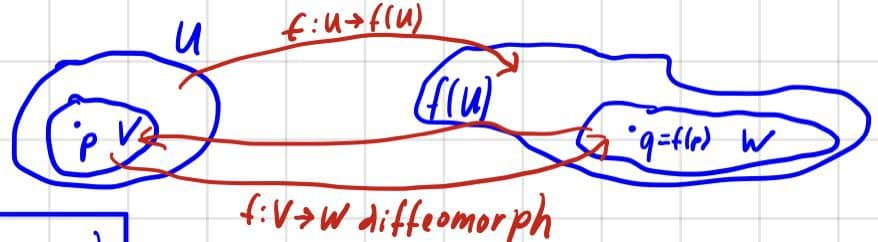
\includegraphics[width=.5\textwidth]{Dateien/09/09Umkehrsatz.jpg}
\end{center}
\end{Satz}
\begin{Beispiel}
{Eine Abbildung{,} die nicht überall umkehrbar ist}
Betrachte die Abbildung $\gvec\mathbb{R}^2\to\mathbb{R}^2,\,\boxed{(u,v)\mapsto\MatrixInline{u^2-v^2\\u v}}$.\\
Die Jacobi-Matrix ist dann $(d\gvec)_{(u,v)}=\MatrixInline{2u&-2v\\u&v}$ mit $\det (d\gvec)_{(u,v)}=2uv+2uv=4uv$.\\
Auf der Einschränkung $V:=\mathbb{R}\setminus\MengeDirekt{0}\times\mathbb{R}\setminus\MengeDirekt{0}$ ist $\gvec$ also ein Diffeomorphismus mit dem Bildbereich $W:=\mathbb{R}\times\mathbb{R}\setminus\MengeDirekt{0}$.\\
Das invertierte Differential ist mit der Cramerschen Regel also
\begin{equation*}
    (d\gvec)^{-1}_{(u,v)}=\frac{1}{4uv}\Matrix{v&2v\\-u&2u}.
\end{equation*}
\end{Beispiel}
\begin{Satz}
{Satz}{Offenheitssatz}
Ist $\fvec:U\to\mathbb{R}^n$ (wobei $U\subseteq\mathbb{R}^n$ offen sei) 
\begin{itemize}
    \item \underline{stetig differenzierbar} und
    \item  $d\fvec_\xvec$ invertierbar $\forall\xvec\in U$.
\end{itemize}
Dann gilt:
$\fvec(U)\subseteq \mathbb{R}^n$ (das Bild von $\fvec$) ist offen.\\
Ist $\fvec$ \underline{injektiv}, so ist $\fvec$ ein Diffeomorphismus für die Einschränkung $\fvec:U\to\fvec(U)$.
\end{Satz}

\begin{Beispiel}
{Ebene Polarkoordinaten}
Aus der Physik kennt ihr bestimmt schon die ebenen Polarkoordinaten:
\begin{equation*}
    \fvec:\mathbb{R}^2\to\mathbb{R}^2,\,(r,\phi)\mapsto\MatrixInline{x\\y}=\MatrixInline{r\cos(\phi)\\r\sin(\phi)}.
\end{equation*}
Diese sind stetig differenzierbar, das Differential ist
\begin{equation*}
    d\fvec_{(r,\phi)}=\MatrixInline{\partial_r(r\cos(\phi))&\partial_\phi(r\cos(\phi))\\\partial_r(r\sin(\phi))&\partial_\phi(r\cos(\phi))}=\MatrixInline{\cos(\phi)&-r\sin(\phi)\\\sin(\phi)&r\cos(\phi)}\tx{ mit }\det(d\fvec)_{(r,\phi)}=r.
\end{equation*}
Wir sehen: $\forall(r,\phi)\in\mathbb{R}_+\setminus\MengeDirekt{0}\times \mathbb{R}$ ist $df_{(r,\phi)}$ \underline{invertierbar}!\\
Laut Umkehrsatz existiert also $\forall\pvec=(r_0,p_0)\in\mathbb{R}_+\setminus\MengeDirekt{0}\times \mathbb{R}$ eine offene Umgebung $V\subseteq\mathbb{R}_+\setminus\MengeDirekt{0}\times \mathbb{R}$, sodass mit $W:=\fvec(V)$ die Abbildung $\fvec:V\to W$ bijektiv ist mit einer stetig differenzierbaren Umkehrabbildung $\fvec^{-1}:W\to V$.\\
Tatsächlich: Definieren wir z. B. $V:=\mathbb{R}_+\setminus\MengeDirekt{0}\times (0,2\pi)$, so ist $\fvec:V\to \fvec(V)$ ein Diffeomorphismus.
\end{Beispiel}
Nun folgt eine andere Herangehensweise:\\
Statt der stetigen Differenzierbarkeit fordern wir nun nur die \underline{Stetigkeit der Umkehrabbildung} und folgern aus der Invertierbarkeit des Differentials, dass ein Diffeomorphismus vorliegt:
\begin{Satz}
{Satz}{Diffeomorphie}
Ist $\fvec:U\to V$ eine \underline{stetig differenzierbare, bijektive} Abbildung zwischen offenen Teilmengen $U$ und $V$ des $\mathbb{R}^n$ mit \underline{stetiger} Umkehrabbildung $\fvec^{-1}:V\to U$, so gilt:\\
Ist $d\fvec_\xvec$ für alle $\xvec\in U$ invertierbar, so ist $\fvec$ ein Diffeomorphismus.
\end{Satz}
\blue{Diffeomorphismen sind wichtig, da sie uns mehrdimensionale Koordinatentransformationen\footnote{Als Beispiel habt ihr ja bestimmt schonmal die ebenen Polar- oder Zylinderkoordinaten behandelt.} liefern, bei denen \textit{keine Informationen} verloren gehen.}
\subsection{Ein neuer Stetigkeitsbegriff}
Für einig der folgenden Anwendungen benötigen wir einen neuen, noch stärkeren Begriff der Stetigkeit. Dieser ist zum Glück aber auch anschaulich verständlich.
\begin{Def}
{Lipschitzstetigkeit}
Auf \underline{normierten} Räumen $V, W$ und $U\subseteq V$ nennen wir eine Funktion $f:U\to W$ \red{lipschitzstetig} auf $U$, wenn eine Konstante $L\geq 0$ existiert, sodass
\begin{equation*}
    \Norm{f(x)-f(y)}\leq L\Norm{x-y}\quad \forall x,y\in U.
\end{equation*}
Diese (nicht eindeutige) Konstante nennen wir \red{Lipschitzkonstante}.
\end{Def}
\blue{Dies ist ein Stetigkeitsbegriff, der eventuell an die kontrahierende Abbildung, die wir für den Banachschen Fixpunktsatz brauchten, erinnert. Eine kontrahierende Abbildung auf normierten Räumen ist eine lipschitzstetige Abbildnung mit einer Lipschitzkonstante $0\leq L<1$.\\
Wir benötigen diesen Stetigkeitsbegriff später noch häufiger, i. d. R. sind hierfür Abschätzungen leichter vorzunehmen. Außerdem findet sich hiermit schnell eine Anwendung des allgemeinen Schrankensatzes.}
\begin{Beispiel}
{Anschauung der Lipschitzstetigkeit}
In 1D kann man sich diesen Begriff anschaulich vorstellen:\\
Damit eine Funktion in einem Punkt lipschitzstetig ist, muss der gesamte Graph der Funktion des an diesem Punkt angelegten Doppelkegels mit der Steigung $\pm L$ sein, wobei $L$ die Lipschitzkonstante mit $L>\frac{\Norm{f(x)-f(y)}}{\Norm{x-y}}\BracedIn{=\frac{\Delta y}{\Delta x}}\,\forall x,y\in \mathbb{R}$ mit $x\neq y$ größer als die stärkste Steigung der Funktion sein muss:
\begin{center}
    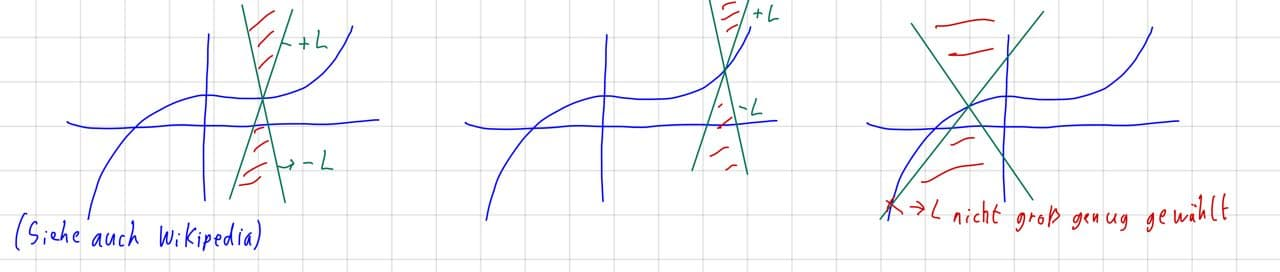
\includegraphics[width=.8\textwidth]{Dateien/09/09Lipschitz.jpg}
\end{center}
Dies ist auf \href{https://de.wikipedia.org/wiki/Lipschitzstetigkeit}{Wikipedia} nochmal schön animiert.
\end{Beispiel}
\begin{Def}
{Konvexität}
\begin{wrapfigure}{r}[0pt]{.35\textwidth}
 \vspace{-15pt}
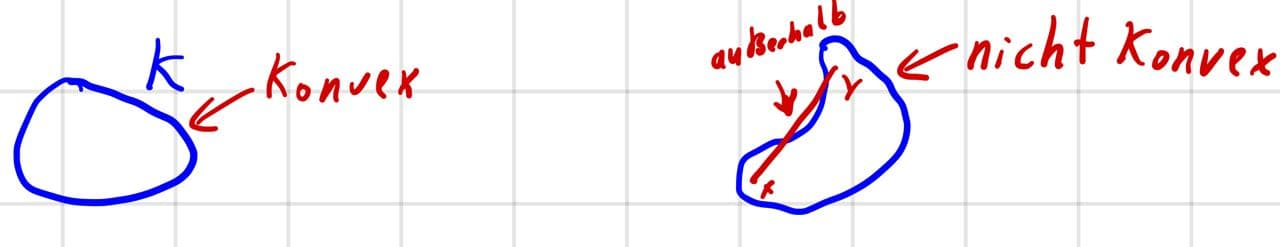
\includegraphics[width=.35\textwidth]{Dateien/09/09Konvex.jpg}
 \vspace{-15pt}
\end{wrapfigure}
Wir nennen eine Teilmenge $K\subseteq U\subseteq\mathbb{R}^n$ \red{konvex}, wenn $\forall x,y\in K$ die Verbindungsstrecke
\begin{equation*}
    V:=\Menge{tx+(1-t)y}{t\in[0,1]}\subseteq K
\end{equation*}
enthalten ist. 
\end{Def}
\begin{Satz}
{Satz}{Schrankensatz}
Sei $\fvec:U\to\mathbb{R}^n$ \underline{stetig differenzierbar}, $K\subseteq U$ \underline{kompakt} und \underline{konvex}.\\
Dann ist $\fvec$ auf $K$ lipschitzstetig mit 
\end{Satz}
\subsection{Der Satz über implizite Funktionen}
Implizit definierte Funktionen kann man sich so vorstellen, dass sie nicht über eine übliche Vorschrift
\begin{equation*}
    F:\,A\rightarrow B, \quad f(x)=y
\end{equation*}
definiert sind, sondern als Lösung einer Gleichung oder eines Gleichungssystems, welches durch eine Funktion $F:\,U\rightarrow\mathbb{R}^n$ mit $U\subseteq\mathbb{R}^m\times\mathbb{R}^n$ gegeben ist. Die implizite Funktion $f$ wird dann durch
\begin{equation*}
    F(x,y,f(x,y)) = 0
\end{equation*}
festgelegt.
\begin{Beispiel}
{Einfache implizit definierte Funktion}
Sei $F:\,\mathbb{R}^2\rightarrow\mathbb{R}, \quad F(x,y)=x^2+y^2-1$. Nun definieren wir implizit die Funktion $g(x)$ durch
\begin{equation*}
    F(x,g(x))=0 \quad \Leftrightarrow\quad x^2+g^2(x)-1=0.
\end{equation*}
Durch Umstellen erhalten wir für $g(x)$ die (explizite) Vorschrift
\begin{equation*}
    g_\pm(x)=\pm\sqrt{1-x^2}.
\end{equation*}
Wir sehen sofort, dass diese Funktion deutlich eingeschränkt ist, nämlich auf das Intervall $x\in[-1,1]$.\\
Außerdem gibt es zwei verschiedene Möglichkeiten, wie sie aussehen kann. Das macht deutlich, dass wir starke Bedingungen an die Funktion stellen müssen, wenn wir eine implizite Definition hinschreiben.
\end{Beispiel}
Natürlich könnt ihr euch zurecht fragen, was das alles soll. Am Ende wird sich herausstellen, dass mit dem Satz über implizite Funktionen ein mächtiges Mittel bereitgestellt wird, um Mannigfaltigkeiten parametrisieren zu können. Dazu werden wir aber erst im nächsten Kapitel kommen, daher müsst ihr den folgenden Satz erstmal schlucken: 

\begin{Satz}{Satz}
    {Satz über implizite Funktionen}
    Beim Satz über implizite Funktionen betrachten wir eine Funktion
    \begin{equation*}
        \fvec:U\rightarrow\mathbb{R}^n \quad U\in\mathbb{R}^m\times\mathbb{R}^n
    \end{equation*}
    und einen Punkt $(\pvec,\qvec)\in U$, sodass also $\pvec\in\mathbb{R}^m$ und $\qvec\in\mathbb{R}^n$. Außerdem definieren wir die Funktion
    \begin{equation*}
        \varphivec:\,\mathbb{R}^n\rightarrow\mathbb{R}^n, \quad \varphivec(y) = f(\pvec,y).
    \end{equation*}
    Nun müssen folgende Voraussetzungen erfüllt sein:
    \begin{enumerate}
        \item $\fvec$ ist \underline{k-mal} differenzierbar (wobei $k\geq 1$)
        \item $\fvec(\pvec,\qvec)=0$
        \item d$\varphivec_\qvec$ ist invertierbar (d. h.: $\det ($d$\varphivec_\qvec)\neq 0$)
    \end{enumerate}
    Ist das der Fall, dann gilt:
    \begin{enumerate}
        \item $\exists$ offene Umgebung $V\subseteq\mathbb{R}^m$ von $\pvec$.
        \item $\exists$ offene Umgebung $W\subseteq\mathbb{R}^n$ von $\qvec$
        \item $\exists$ \underline{k-mal} stetig differenzierbare Funktion $\gvec:V\rightarrow W$ sodass
        \begin{equation*}
            \forall(\xvec,\yvec)\in V\times W: \qquad f(\xvec,\yvec) = 0 \quad \Leftrightarrow \yvec = \gvec(\xvec) 
        \end{equation*}
    \end{enumerate}
    Dies kann man auch anders formulieren. Betrachte dazu die Mengen
    \begin{align*}
        N_f(0)&=\Menge{\xvec\in\mathbb{R}^m\times\mathbb{R}^n}{\fvec(\xvec)=0} \\
        \graph(\gvec)&=\Gamma_\gvec=\Menge{(\xvec,\gvec(\xvec))\in V\times W}{\xvec\in V}.
    \end{align*}
    Dann gilt
    \begin{equation*}
        N_f(0)\cap V\times W = \graph(\gvec).
    \end{equation*}
    Das schreit doch förmlich nach Beispielen!
\end{Satz}

\begin{Beispiel}
    {Ausführliches Anwendungsbeispiel für den Satz über implizite Funktionen}
    Wir betrachten wieder die Funktion $f:\mathbb{R}^2\rightarrow\mathbb{R}, f(x,y)=x^2+y^2-1$. Für den benötigten Punkt wählen wir $(p,q)=(0,1)$. \\
    
    Zuerst definieren wir die Funktion
    \begin{equation*}
        \varphi:\,\mathbb{R}\rightarrow\mathbb{R}, \quad \varphi(y)=f(p,y)=0^2+y^2-1=y^2-1.
    \end{equation*}
    und überprüfen gemäß des Satzes über implizite Funktionen:
    \begin{enumerate}
        \item $f$ ist zusammengesetzt aus $\infty$-oft differenzierbaren Funktionen, also ist $f$ selbst $\infty$-oft differenzierbar.
        \item $f(p,q)=f(0,1)=0^2+1^2-1=0$.
        \item Ist d$\varphi_1$ invertierbar?\\
        d$\varphi_y$=$\partial_y\varphi=2y \quad \implies \quad$d$\varphi_q=$d$\varphi_1=2 \quad \implies \quad \det($d$\varphi_1)=2\neq0$\\
        $\implies \quad$d$\varphi_1$ ist invertierbar.
    \end{enumerate}
    Alle Voraussetzungen sind erfüllt, es existieren also die entsprechenden Mengen $V$ und $W$ sowie die Funktion $g$ und wir können wieder schreiben
    \begin{equation*}
        f(x,g(x))=0 \quad \Leftrightarrow \quad g_\pm(x)=\pm\sqrt{1-x^2} \quad (g:V\rightarrow W).
    \end{equation*}
    Da $(p,q)=(0,1)\in\graph(g)=\Menge{(x,g(x))\in V\times W}{x\in\mathbb{R}}$ gilt, ist die Funktion durch
    \begin{equation*}
        g_+(x)=\sqrt{1-x^2}
    \end{equation*}
    eindeutig bestimmt. Nun existieren für $g_+(x)$ nur Lösungen im Intervall $[-1,1]$. Da $g_+$ $\infty$-oft differenzierbar sein soll, dürfen die Randpunkte $x_1=-1$ und $x_2=1$ nicht in der Definitionsmenge $V$ enthalten sein. Daraus folgt $V=(-1,1)$.\\
    Die (offene) Bildmenge $W$ kann man dann wählen durch $W=(0,a)$ mit einer beliebigen reellen Zahl $a>1$. \\
    Somit haben wir die implizite Funktion gefunden:
    \begin{equation*}
        g_+:\,(-1,1)\rightarrow (0,a), \quad x\mapsto\sqrt{1-x^2} \quad (a>1).
    \end{equation*}
    Natürlich muss die Bildmenge in diesem Beispiel nicht zwangsläufig offen sein, aber um hier den Satz über implizite Funktionen nachvollziehen zu können, haben wir das getan. \\
    
    \textbf{Anmerkung}:\\
    Die Menge $N_f(0)$ ist in diesem Beispiel
    \begin{equation*}
        N_f(0)=\Menge{(x,y)\in\mathbb{R}^2}{x^2+y^2=1}=S^1,
    \end{equation*}
    also der Einheitskreis. Wir können nun die folgende Zeichnung für die von uns gefundenen Mengen $V=(-1,1)$ und $W=(0,a)$ ($a>1$) betrachten:
    \begin{center}
        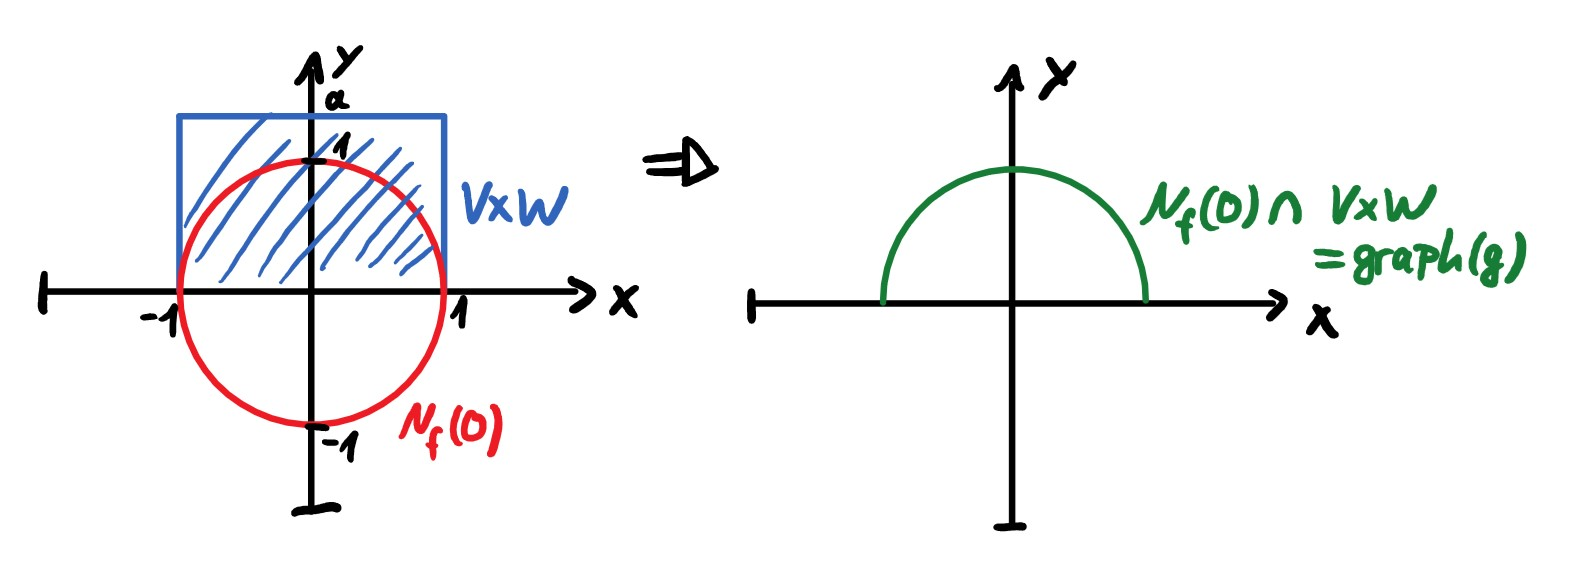
\includegraphics[width=.8\textwidth]{Dateien/09/09BeispielImpliziteFunktionen.jpg}
    \end{center}
    Wir werden im nächsten Kapitel feststellen, dass man den Einheitskreis $S^1$ als Untermannigfaltigkeit verstehen kann.\\
    Durch die Menge $\graph(g)$ ist dann eine lokale Parametrisierung (= Karte) um den Punkt $(p,q)=(0,1)$ gegeben. Diese parametrisiert aber nur den oberen Halbkreis, für den Unteren ist die zweite Lösung $g_-$ herzunehmen.
\end{Beispiel}
\begin{Beispiel}
    {Weiteres Beispiel zum Satz über implizite Funktionen}
    Zur Abwechslung betrachten wir mal eine etwas andere Funktion, nämlich $f:\mathbb{R}^2\rightarrow\mathbb{R}, \quad f(x,y)=x-y^3$ um den Punkt $(p,q)=(1,1)$. \\
    
    Wieder definieren wir zuerst die Funktion
    \begin{equation*}
        \varphi:\mathbb{R}\rightarrow\mathbb{R}, \quad \varphi(y)=f(p,y)=1-y^3
    \end{equation*}
    und überprüfen gemäß des Satzes über implizite Funktionen:
    \begin{enumerate}
        \item Da $f$ sich aus $\infty$-oft differenzierbaren Funktionen zusammensetzt, ist $f$ ebenfalls $\infty$-oft differenzierbar.
        \item $f(p,q)=f(1,1)=0$.
        \item d$\varphi_y$=$\partial_y\varphi=-3y^2 \quad \Rightarrow \quad$d$\varphi_q=$d$\varphi_1=-3 \quad \Rightarrow \quad \det($d$\varphi_1)=-3\neq0 \quad \Rightarrow \quad$d$\varphi_1$ ist invertierbar.
    \end{enumerate}
    Die Voraussetzungen sind also erfüllt. Daraus können wir folgern:
    \begin{equation*}
        f(x,g(x))=x-g^3(x)=0\quad \Leftrightarrow \quad g(x)=\sqrt[3]{x}.
    \end{equation*}
    Diese Funktion ist differenzierbar auf $V=\mathbb{R}_+$ und zudem bijektiv, wenn wir für die Bildmenge ebenfalls $W=\mathbb{R}_+$ wählen. Somit haben wir gefunden:
    \begin{equation*}
        g:\,V\rightarrow W, \quad g(x)=\sqrt[3]{x}.
    \end{equation*}
\end{Beispiel}

\subsubsection{Differentiale von impliziten Funktionen}
Nun werden wir uns an eine etwas schwierigere Übung wagen, nämlich das Differential einer impliziten Funktion aufzustellen. Das Tolle ist nämlich, dass wir das tun können, ohne jemals eine explizite Vorschrift hinschreiben zu müssen. Was daran der Vorteil ist? Nun ja, wir haben uns bis jetzt nur sehr einfache Beispiele angeschaut, bei denen die implizite Funktion schnell gefunden war. Bei Gleichungssystemen höherer Ordnung wird das schon schwieriger. \\

Wir fangen direkt ganz allgemein mit einer Funktion $\fvec:\,\mathbb{R}^m\times\mathbb{R}^n\rightarrow\mathbb{R}^n$ an, von der wir voraussetzen dass sie an einem Punkt $(\pvec,\qvec)$ die Voraussetzungen für den Satz über implizite Funktionen erfülle. Sei $\gvec:\,V\rightarrow W$ nun diese implizite Funktion, es gelte also $\fvec(\xvec,\gvec(\xvec))=0$. \\
Man definiert nun die Hilfsfunktion
\begin{equation*}
    \hvec:\,\mathbb{R}^m\rightarrow\mathbb{R}^m\times\mathbb{R}^n, \quad \hvec(\xvec)=(\xvec,\gvec(\xvec)).
\end{equation*}
und nutzt aus, dass die Funktion $\fvec(\xvec,\gvec(\xvec))$ \underline{per Definition die Nullfunktion ist}!\\
Dadurch können wir nämlich unter Ausnutzung der Kettenregel schreiben:
\begin{equation*}
    0=\text{d}(0)=\text{d}\fvec(\xvec,\gvec(\xvec))=\text{d}\fvec(\hvec(\xvec))=\text{d}\fvec_{\hvec(\xvec)}\circ\text{d}\hvec_\xvec.
\end{equation*}
Diese Gleichung können wir nun ein wenig weiter massieren\footnote{Fragt uns bitte nicht, woher wir diese komischen Mathetermini haben. Alternativ könnten wir auch \textit{verarzten}, \textit{bearbeiten}, \textit{streicheln} oder Seltsameres anbieten.}, wenn wir die Matrizenschreibweise benutzen. Ab jetzt wird es allerdings eine Indexschlacht, das ist leider nicht ganz zu vermeiden:
\begin{equation*}
    0=\Big[ (\partial_j F_i)(\hvec(\xvec)) \Big]_{\substack{1\leq i\leq n \\ 1 \leq j \leq m+n}}\cdot \Big[(\partial_j h_i)(\xvec))\Big]_{\substack{1 \leq i \leq m+n \\ 1 \leq j \leq m}} = \Big[ \sum_{k=1}^{m} (\partial_k F_i)(\hvec(\xvec))\cdot(\partial_j h_k)(\xvec) \Big]_{\substack{1\leq i\leq n \\ 1 \leq j \leq m}}
\end{equation*}
Im letzten Schritt haben wir eine ganz normale Matrixmultiplikation durchgeführt, sollte euch die Summenschreibweise nicht mehr vertraut sein schaut nochmal ins Skript von Mathe 1! Im nächsten Schritt betrachten wir die Abbildung $(\partial_j h_k)(\xvec))$ genauer. Für $1\leq k \leq m$ ist diese schlicht:
\begin{equation*}
    (\partial_j h_k)(\xvec))=(\partial_j x_k)(\xvec)=\delta_{jk} \quad (1\leq k\leq m).
\end{equation*}
Für $m+1 \leq k \leq m+n$ gilt jedoch
\begin{equation*}
    (\partial_j h_k)(\xvec))=(\partial_j g_{k-m}(\xvec)) \quad (m+1 \leq k \leq m+n).
\end{equation*}
Teilen wir die Summe in unserer Gleichung entsprechend auf und setzen den ganzen Spaß ein, dann erhalten wir
\begin{align*}
    0&=\Big[ \sum_{k=1}^m (\partial_k F_i)(\hvec(\xvec))\cdot\delta_{jk} + \sum_{k=m+1}^{m+n} (\partial_k F_i)(\hvec(\xvec))\cdot(\partial_j g_{k-m})(x))\Big]_{\substack{1\leq i\leq n \\ 1\leq j\leq m}} \\ &= \Big[ (\partial_j F_i)(\hvec(\xvec)) + \sum_{k=1}^{n} (\partial_{k+m} F_i)(\hvec(\xvec))\cdot(\partial_j g_{k})(\xvec))\Big]_{\substack{1\leq i\leq n \\ 1\leq j\leq m}}.
\end{align*}
Die Komponenten $(\partial_j g_k)(\xvec)$ des Differentials sind somit über folgende Gleichung bestimmt, die ihr auch so in eurem Skript stehen habt:
\begin{equation*}
    \sum_{k=1}^{n} (\partial_{k+m} F_i)(\xvec,\gvec(\xvec))\cdot(\partial_j g_{k})(\xvec) = - (\partial_j F_i)(\xvec,\gvec(\xvec)).
\end{equation*}
Hierbei haben wir übrigens auch wieder $\hvec(\xvec)=(\xvec,\gvec(\xvec))$ eingesetzt. \\

Ja, diese Herleitung ist nicht ganz einfach, besonders wenn man mit dieser Indexschreibweise noch nicht so vertraut ist. Ihr seid aber bereits im zweiten Semester, deswegen könnt ihr durchaus mal mutig sein und versuchen, die Rechnung nachzuvollziehen. Solltet ihr jedoch verzweifelt auf diese Seite starren und gar nicht mehr wissen wo hinten und vorne ist, dann braucht ihr trotzdem nicht aufzugeben. In der Regel wird diese Rechnung für Spezialfälle genutzt und braucht diese allgemeine Formel nicht heranzuziehen. Genau das wollen wir jetzt aber einmal machen.

\begin{Beispiel}
    {Das Differential einer impliziten Funktion}
    Wir betrachten die folgende Funktion:
    \begin{equation*}
        f:\mathbb{R}^3\rightarrow\mathbb{R}, \quad f(x,y,z)=z^3+2xy-4xz+2y-1
    \end{equation*}
    und die zugehörige implizite Funktion $g(x,y)$, sodass
    \begin{equation*}
        f(x,y,g(x,y))=0
    \end{equation*}
    Wie lautet nun das Differential am Punkt $(x,y)=(0,1)$? Dazu stellen wir zunächst die Hilfsfunktion $h$ auf:
    \begin{equation*}
        \hvec:\mathbb{R}^2\rightarrow\mathbb{R}^3, \quad \hvec(x,y)=(x,y,g(x,y))
    \end{equation*}
    und nutzen aus, dass das Differential von $f(x,y,g(x,y))$ per Definition $0$ ist:
    \begin{align*}
        0&=(\text{d}f)(x,y,g(x,y))=(\text{d}f)(\hvec(x,y))=\text{d}f_{\hvec(x,y)}\circ\text{d}\hvec_{(x,y)} \\ &= \Matrix{\partial_1 f & \partial_2 f & \partial_3 f}_{\hvec(x,y)}\Matrix{\partial_1 h_1 & \partial_2 h_1 \\ \partial_1 h_2 & \partial_2 h_2 \\ \partial_1 h_3 & \partial_2 h_3}_{(x,y)} \\ &= \Matrix{\partial_1 f & \partial_2 f & \partial_3 f}_{\hvec(x,y)}\Matrix{1 & 0 \\ 0 & 1 \\ \partial_1 g & \partial_2 g}_{(x,y)} \\ &= \Matrix{(\partial_1 f)(\hvec(x,y))+(\partial_3 f)(\hvec(x,y))(\partial_1 g)(x,y) \\ (\partial_2 f)(\hvec(x,y))+(\partial_3 f)(\hvec(x,y))(\partial_2 g)(x,y)}^T \\ &=\Matrix{\partial_1 f \\ \partial_2 f}^T_{\hvec(x,y)} + (\partial_3 f)(\hvec(x,y))\Matrix{\partial_1 g \\ \partial_2 g}^T_{(x,y)}
    \end{align*}
    Stellen wir diese Gleichung um, erhalten wir also
    \begin{equation*}
        \text{d}g_{(x,y)} = \Matrix{\partial_1 g & \partial_2 g}_{(x,y)} = -\Matrix{(\partial_1 f)(x,y,g(x,y)) \\ (\partial_2 f)(x,y,g(x,y))}^T\cdot\frac{1}{(\partial_3 f)(x,y,g(x,y))}.
    \end{equation*}
    Im finalen Schritt müssen wir nur noch $f$ und $(x,y)=(0,1)$ einsetzen. Wir stellen zunächst fest, dass
    \begin{equation*}
        0=f(0,1,g(0,1))=g^3(0,1)+2-1 \quad \Leftrightarrow \quad g(0,1)=-1
    \end{equation*}
    Daraus folgt:
    \begin{align*}
        \partial_1 f &= 2y-4z \quad \Rightarrow \quad (\partial_1 f)(0,1,-1)=6 \\
        \partial_2 f &= 2x+2 \quad \Rightarrow \quad (\partial_2 f)(0,1,-1)=2 \\
        \partial_3 f &= 3z^2-4x \quad \Rightarrow \quad (\partial_3 f)(0,1,-1)=3 
    \end{align*}
    und damit weiter:
    \begin{align*}
        (\partial_1 g)(0,1) &= -\frac{(\partial_1 f)(0,1,-1)}{(\partial_3 f)(0,1,-1)} = -2 \\
        (\partial_2 g)(0,1) &= -\frac{(\partial_2 f)(0,1,-1)}{(\partial_3 f)(0,1,-1)} = -\frac{2}{3}.
    \end{align*}
    Wir haben also endlich das gewünschte Differential gefunden:
    \begin{equation*}
        \text{d}g_{(0,1)}=\Matrix{(\partial_1 g)(0,1) & (\partial_2 g)(0,1)} = \Matrix{-2 & -\frac{2}{3}}.
    \end{equation*}
    Auch das ist zugegebenermaßen eine etwas gewöhnungsbedürftige Rechnung, aber sie ist schon mal deutlich übersichtlicher als die Herleitung der allgemeinen Formel. Nehmt euch ruhig die Zeit dafür und schaut euch jeden Schritt genau an, dann sollten die Übungsaufgaben dazu durchaus schaffbar sein :).
\end{Beispiel}

\subsection{Differenzierbare Abbildungen}
Wir starten dieses Thema mit einer wichtigen Wiederholung - der Rang von Abbildungen wird uns helfen, diese genauer zu charakterisieren.
\begin{Wiederholung}
{Rang einer Matrix}
Der \red{Rang} einer Matrix entspricht der \underline{Anzahl an linear unabhängigen Spalten} (bzw. Zeilen) der Matrix.\\
Also ist der Rang die Anzahl der Zeilen, die nach Anwendung des Gauß-Algorithmus nicht 0 werden.
\end{Wiederholung}
\begin{Wiederholung}
{Spaltenrang = Zeilenrang}
Es gilt $\rg(A)=\rg(A^T)$.
\end{Wiederholung}
\begin{Beispiel}
{Wiederholendes Beispiel zum Rang}
Die folgende Matrix kann aufgrund des Satzes über das Transponieren maximal $\rg C\leq 2$ haben:
\begin{equation*}
    C=\Matrix{1&2\\3&4\\5&6}.
\end{equation*}
Betrachten wir $C^T$, so sehen wir:
\begin{equation*}
    C^T=\Matrix{1&3&5\\2&4&6}\overset{(II)-2(I)}{\to}\Matrix{1&3&5\\0&-2&-4}\Rightarrow\rg C^T=\rg C=2,
\end{equation*}
weil die Matrix ja zwei linear unabhängige Zeilen hat.
\end{Beispiel}
Den Rang einer \underline{linearen} Abbildung $F$ hatten wir über den Rang der darstellenden Matrix definiert. Wie sieht das aber jetzt für allgemeinere (vielleicht nicht-lineare) Abbildungen zwischen mehrdimensionalen Vektorräumen aus? Tatsächlich besteht eine Möglichkeit, die darstellende Matrix einer linearen Abbildung $\mathbb{R}^m\to\mathbb{R}^n$ bzgl. der kanonischen Basis zu finden, darin, einfach das Differential zu bilden! Dieses ist für lineare Abbildungen überall konstant.\\
Im Folgenden wird das ähnlich sein, allerdings hängen die darstellenden Matrizen von allgemeineren Abbildungen i. d. R. noch von $\xvec$ ab.\\
\red{Achtung!\\
Verwirrenderweise werden im \Skript{} nun auf einmal Abbildungen aus $\mathbb{R}^m$ nach $\mathbb{R}^n$ (also genau umgekehrt wie bisher) verwendet!\\
Wir machen das hier nun auch so, aber immer aufpassen, für welche Räume die Dimensionen stehen!}
\begin{Def}
{Rang einer Abbildung}
Für eine Funktion $f:U\to\mathbb{R}^n$ ($U\subseteq\mathbb{R}^m$) definieren wir für jeden Punkt $\pvec\in U$ den \red{Rang} von $f$ als den \underline{Rang des Differentials} in $\pvec$:
\begin{equation}
    \rg(f)_\pvec:=\rg(df_\pvec)\leq\min(m,n).
\end{equation}
Er ist stets kleiner als das Minimum aus den Dimensionen (s. o.).\\
Da $\rg(f)$ von $\pvec$ abhängt, können wir ihn auch als Abbildung
\begin{equation}
    \rg(f):U\to\MengeDirekt{0,1,\ldots,\min(m,n)}\subseteq\mathbb{N}
\end{equation}
auffassen.
\end{Def}
\begin{Beispiel}
{Rang irgendeiner Abbildung}
Wir betrachten die Abbildung $f:\mathbb{R}^3\to\mathbb{R}^2,\,\boxed{f(x,y,z)=\MatrixInline{x^2+2y\\2yz^2+2x}}$.\\
Das Differential dieser Abbildung ist
\begin{equation*}
    df_{(x,y,z)}=\Matrix{2x&2&0\\2&2z^2&4yz}.
\end{equation*}
Wir können uns nun die Frage stellen, für welche $\pvec=(x,y,z)$ diese Matrix einen Rang von 2 oder sogar einen geringeren Rang hat.\\
Hier sehen wir recht offensichtlich: Sobald $y=0$ und gleichzeitig $x=z^2$ sind, sind die beiden Zeilen linear abhängig, wir haben also
\begin{equation*}
    \rg(f)=\Cases{1\quad & \xvec\in M:=\Menge{(x,y,z)\in\mathbb{R}}{x=z^2\land y=0}\\ 2&\xvec\in\mathbb{R}^3\setminus M}
\end{equation*}
\red{Der Rang kann also je nach betrachtetem Punkt variieren!}
\end{Beispiel}
\subsubsection{Abbildungen von konstantem Rang}
Falls der Rang \red{konstant} ist, unterscheiden wir zwischen den folgenden Spezialfällen:
\begin{Def}
{Immersion}
Ist $\rg(f)=m\,\forall \pvec\in U$, d. h. die Abbildung hat den konstanten Rang der Dimension des \underline{Urbildraums}, so sagen wir, dass $f$ eine \red{Immersion} ist.\\
Das Differential $df:U\to\mathbb{R}^n$ ist dann injektiv. 
\end{Def}
\begin{Def}
{Submersion}
Ist $\rg(f)=n\,\forall \pvec\in U$, d. h. die Abbildung hat den konstanten Rang der Dimension des \underline{Bildraumes}, so sagen wir, dass $f$ eine \red{Submersion} ist.\\
Das Differential $df:U\to\mathbb{R}^n$ ist dann surjektiv.
\end{Def}
\begin{Wiederholung}
{$C^k$-Abbildungen}
$k$-fach \underline{stetig differenzierbare} Abbildungen bezeichnen wir von nun an als \red{$C^k$-Abbildungen}, wobei $k\in N\cup\infty$.
\end{Wiederholung}
\begin{Def}
{$C^k$-Diffeomorphismen}
$C^k$-Abbildungen $f:U\to V$, die bijektiv sind und deren Umkehrabbildungen auch $C^k$ sind, nennen wir \red{$C^k$-Diffeomorphismen}.
\end{Def}
\begin{Beispiel}
{Abbildung von konstantem Rang?}
Wir betrachten $f:\mathbb{R}^2\to\mathbb{R}^3\,\boxed{f(x,y)=\MatrixInline{e^x+y\\e^y\\-x^2+y}}$.\\
Diese Abbildung hat mit
\begin{equation*}
    df_{(x,y)}=\Matrix{e^x&1\\0&e^y\\-2x&1}
\end{equation*}
den konstanten Rang $2$.\\
\blue{(Der einzige problematische Punkt wäre $(x,y)=(0,y)$, denn hier ist
\begin{equation*}
    df^T_{(x,y)}=\Matrix{e^0&0&-2\cdot 0\\1&e^y&1}=\Matrix{1&0&0\\1&e^y&1},
\end{equation*}
doch auch hier ist $\rg(df)=2$, denn durch den Gauß-Algorithmus lässt sich keine Nullzeile erzeugen.}\\
Somit ist $f$ eine \underline{Immersion}.
\end{Beispiel}
Nächste Woche gibt es weitere Beispiele!\\
\textbf{Ausblick}:\\
Für die kommenden Überlegungen werden wir das \textit{überall}, das für Immersionen und Submersionen gefordert wird, zum Teil auf lokale Umgebungen einschränken.\\
Im \Skript{} sind auch hier ein paar anschauliche Beispiele, die ihr auf jeden Fall ansehen und bestenfalls verstehen solltet.

\Tipps{10}{
\begin{enumerate}
    \item Beide Differentialgleichungen solltet ihr gut lösen können, indem ihr den entsprechenden Typ identifiziert und den dazugehörigen Satz aus der Vorlesung anwendet.\\
    Beispiele dazu werdet ihr in unseren kommenden Notizen finden, die wir hochladen, sobald wir die Zeit finden, sie zu schreiben.
    \item Über lineare Differentialgleichungssysteme hatten wir im Tutorium noch nicht gesprochen. Die entscheidende Gleichung findet ihr auf Folie 400 im Skript. Erinnert euch in diesem Zusammenhang auch an den Basistransformationssatz, den wir ganz am Anfang einmal im Tutorium besprochen haben ($D_A=S^{-1}AS$, wobei die Spalten von $S$ die Eigenvektoren von $A$ enthalten). 
    \item Hier wendet ihr zwei Sätze aus der Vorlesung über Untermannigfaltigkeiten an. Zu diesem Aufgabentyp haben wir auch im Tutorium schon einiges gesagt.
    \item Denkt daran, zuerst zu zeigen, dass die Randbedingung $f(x,y,z):=xy-z^{-1}$ durch $f^-1(0)$ eine Untermannigfaltigkeit definiert - wie zeigt man nochmal, dass eine Abbildung eine Submersion ist? Dann könnt ihr euch an dem Satze auf Folie 321 entlanghangeln. Um zu zeigen, dass das Kriterium hinreichend ist, müsst ihr eine geeignete kompakte Menge definieren und euch überlegen, was stetige Funktionen auf kompakten Mengen so anstellen. Den entscheidenden Satz findet ihr im Kapitel über topologische Grundbegriffe und Vollständigkeit (Teil 2).\\
    In den Notizen von nächster Woche werdet ihr dazu auch ein Beispiel finden, das wir wahrscheinlich Montag hochladen werden.
    \item Für diesen Aufgabentyp findet ihr in diesen Notizen ausführlich Beispiele. Versteht die Schritte und hangelt euch mit diesen durch die Aufgabe, dann schafft ihr das!
\end{enumerate}}